% Circonferenza goniometrica: angoli notevoli e coordinate esatte
% Print-first reference chart with a radial structure: every notable angle
% owns a ray from the origin, and everything about that angle is read along
% the ray, from the centre outwards:
%     origin -> ray -> degrees -> radians -> point P -> (cos, sin)
%
% Placement model (all radii in units of the circle radius):
%   - the 12 non-cardinal directions share one rule: labels are centred on
%     their own ray and rotated along it (angle theta in the right half-plane,
%     theta-180 in the left one, so no text is upside down); a white halo
%     interrupts the ray behind the label;
%   - all degrees sit on one ring, all radians on another (15 deg leaves
%     room for both at this scale); each quadrant is the mirror image of Q1;
%   - coordinates start just outside the point and grow outwards along the
%     ray: radial text spends radial space, which is free, not tangential
%     space, which is what 15 deg leaves scarce;
%   - the four cardinal directions have their own rule: horizontal labels on
%     the counterclockwise side of their axis (a quarter turn maps each one
%     onto the next);
%   - hand corrections go in the `deg <a>` / `rad <a>` / `crd <a>` keys.
% Colour marks the family (pi/6 blue, pi/4 dark amber, axes black); it is
% redundant with the values, so the figure reads the same in grayscale.
% The figure is language-neutral (math only).
% OrbBits TikZ conventions: see docs/style/tikz.md
\documentclass[tikz,border=10pt]{standalone}
\usepackage{amsmath,amssymb}
\usetikzlibrary{arrows.meta}

% Project palette (keep colours semantic, not decorative)
\definecolor{orbPrimary}{HTML}{1F5FBF}
\definecolor{orbAccent}{HTML}{E0A100}
\definecolor{orbMuted}{HTML}{7A7A7A}

% Families of directions
\colorlet{fam6}{orbPrimary}          % multiples of 30 deg (pi/6)
\colorlet{fam4}{orbAccent!70!black}  % odd multiples of 45 deg (pi/4)

% Radial rings (units of the radius): centre of the label on its ray
\def\rDeg{0.52}    % degrees
\def\rRad{0.80}    % radians
\def\gapCrd{0.045}                      % point -> start of the coordinates

\begin{document}
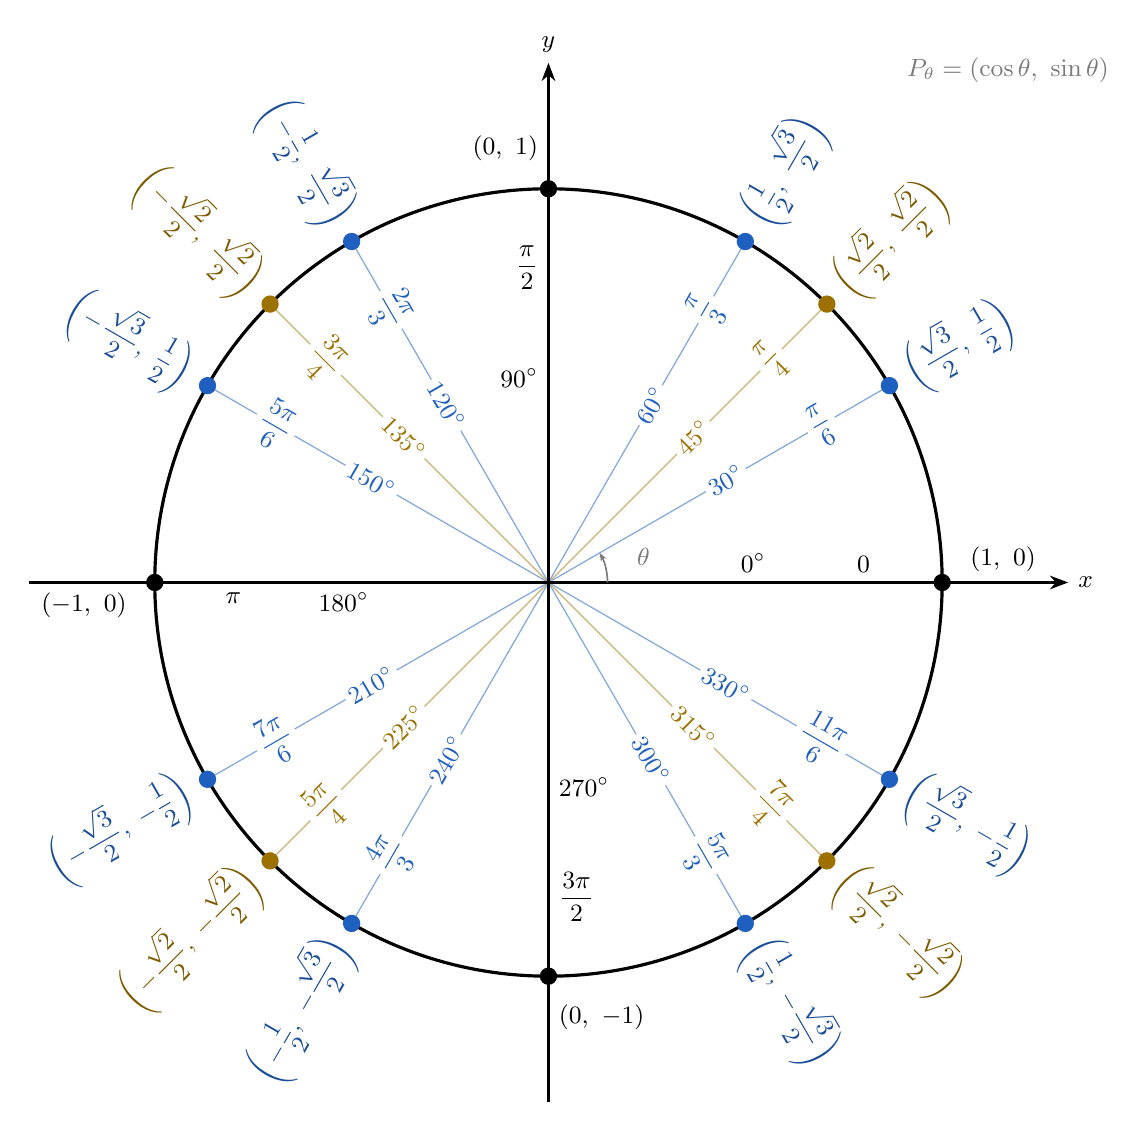
\begin{tikzpicture}[
    >=Stealth,
    scale=5,                    % geometry in units of the radius; text stays \small
    line width=0.9pt,
    every node/.style={font=\small},
    halo/.style={fill=white, inner sep=1.5pt},
    ray/.style={line width=0.45pt},
    % ---- manual overrides (layout, not mathematics), e.g.
    %      crd 60/.style={xshift=2pt},  rad 45/.style={yshift=-1pt}
    % none needed at present: the rings clear every cluster ----
  ]

  % ---- rays of the non-cardinal directions (under everything else) ----
  \foreach \a/\f in {30/6,45/4,60/6,120/6,135/4,150/6,210/6,225/4,240/6,300/6,315/4,330/6}
    \draw[ray, fam\f!55] (0,0) -- (\a:1);

  % ---- axes, calibrated by the circle itself: the +/-1 points are on them ----
  \draw[black, line width=0.8pt, ->] (-1.32,0) -- (1.32,0) node[right] {$x$};
  \draw[black, line width=0.8pt, ->] (0,-1.32) -- (0,1.32) node[above] {$y$};

  % ---- unit circle ----
  \draw[black, line width=1.15pt] (0,0) circle (1);

  % ---- the reading convention, once: theta from the positive x-axis ----
  \draw[orbMuted, line width=0.6pt, -{Stealth[length=3pt]}]
    (0:0.15) arc[start angle=0, end angle=30, radius=0.15];
  \node[text=orbMuted, inner sep=1pt, name=theta] at (15:0.25) {$\theta$};

  % ---- the twelve non-cardinal directions ----
  % angle / radians / cos / sin / family (6 = pi/6, 4 = pi/4)
  \foreach \a/\rad/\cx/\cy/\f in {
      30/{\dfrac{\pi}{6}}/{\dfrac{\sqrt{3}}{2}}/{\dfrac{1}{2}}/6,
      45/{\dfrac{\pi}{4}}/{\dfrac{\sqrt{2}}{2}}/{\dfrac{\sqrt{2}}{2}}/4,
      60/{\dfrac{\pi}{3}}/{\dfrac{1}{2}}/{\dfrac{\sqrt{3}}{2}}/6,
      120/{\dfrac{2\pi}{3}}/{-\dfrac{1}{2}}/{\dfrac{\sqrt{3}}{2}}/6,
      135/{\dfrac{3\pi}{4}}/{-\dfrac{\sqrt{2}}{2}}/{\dfrac{\sqrt{2}}{2}}/4,
      150/{\dfrac{5\pi}{6}}/{-\dfrac{\sqrt{3}}{2}}/{\dfrac{1}{2}}/6,
      210/{\dfrac{7\pi}{6}}/{-\dfrac{\sqrt{3}}{2}}/{-\dfrac{1}{2}}/6,
      225/{\dfrac{5\pi}{4}}/{-\dfrac{\sqrt{2}}{2}}/{-\dfrac{\sqrt{2}}{2}}/4,
      240/{\dfrac{4\pi}{3}}/{-\dfrac{1}{2}}/{-\dfrac{\sqrt{3}}{2}}/6,
      300/{\dfrac{5\pi}{3}}/{\dfrac{1}{2}}/{-\dfrac{\sqrt{3}}{2}}/6,
      315/{\dfrac{7\pi}{4}}/{\dfrac{\sqrt{2}}{2}}/{-\dfrac{\sqrt{2}}{2}}/4,
      330/{\dfrac{11\pi}{6}}/{\dfrac{\sqrt{3}}{2}}/{-\dfrac{1}{2}}/6}
  {
    % left half-plane: turn the text by 180 deg so it never reads upside down
    \pgfmathtruncatemacro{\isLeft}{(\a > 90) && (\a < 270)}
    \ifnum\isLeft=1
      \pgfmathsetmacro{\rot}{\a-180}\def\crdAnchor{east}
    \else
      \pgfmathsetmacro{\rot}{\a}\def\crdAnchor{west}
    \fi

    \node[halo, text=fam\f, rotate=\rot, name=deg-\a, deg \a/.try]
      at (\a:\rDeg) {$\a^\circ$};
    \node[halo, text=fam\f, rotate=\rot, name=rad-\a, rad \a/.try]
      at (\a:\rRad) {$\rad$};
    \fill[fam\f] (\a:1) circle (0.022);
    \node[text=fam\f!80!black, rotate=\rot, anchor=\crdAnchor, inner sep=1pt,
          name=crd-\a, crd \a/.try]
      at (\a:1+\gapCrd) {$\left(\cx,\ \cy\right)$};
  }

  % ---- the four cardinal directions: horizontal, counterclockwise side ----
  % angle / radians / coordinates / anchor of the labels / direction of the side
  \foreach \a/\rad/\crd/\lAnchor/\cAnchor in {
      0/0/{(1,\ 0)}/south/south west,
      90/{\dfrac{\pi}{2}}/{(0,\ 1)}/east/south east,
      180/\pi/{(-1,\ 0)}/north/north east,
      270/{\dfrac{3\pi}{2}}/{(0,\ -1)}/west/north west}
  {
    \node[anchor=\lAnchor, name=deg-\a] at (\a:\rDeg) {$\a^\circ$};
    \node[anchor=\lAnchor, name=rad-\a] at (\a:\rRad) {$\rad$};
    \fill[black] (\a:1) circle (0.022);
    \node[anchor=\cAnchor, name=crd-\a] at (\a:1+\gapCrd) {$\crd$};
  }

  % ---- the one general annotation ----
  \node[text=orbMuted, anchor=north east, name=annot] at (1.45,1.36)
    {$P_\theta = (\cos\theta,\ \sin\theta)$};
\end{tikzpicture}
\end{document}
